% AVA Internal Report #3 — PyTICS Ensemble Calibration Update
\documentclass[10pt,a4paper,oneside]{report}
\usepackage[T1]{fontenc}
\usepackage{tgtermes}
\usepackage{mathptmx}
\usepackage[a4paper,top=2.3cm,bottom=2.5cm,left=2.4cm,right=2.4cm,headsep=0.6cm]{geometry}
\usepackage{graphicx}
\usepackage{amsmath}
\usepackage{booktabs}
\usepackage{tabularx}
\usepackage{longtable}
\usepackage{xcolor}
\usepackage[hyphens]{url}
\usepackage{listings}
\usepackage{mdframed}
\usepackage[font=small,labelfont=bf,labelsep=period,justification=justified,singlelinecheck=false]{caption}
\usepackage{titlesec}
\usepackage{fancyhdr}
\usepackage{tikz}
\usetikzlibrary{positioning,calc}
\usepackage[colorlinks=true,linkcolor={blue!60!black},citecolor={blue!60!black},urlcolor={blue!60!black}]{hyperref}
\PassOptionsToPackage{hyphens}{url}

%% AVA colours
\definecolor{avaInkBlue}{RGB}{26,58,92}
\definecolor{avaAbyss}{RGB}{10,22,40}
\definecolor{avaGold}{RGB}{212,160,23}
\definecolor{avaMidBlue}{RGB}{14,44,80}
\definecolor{avaCopper}{RGB}{200,90,0}
\definecolor{avaCodeBG}{RGB}{238,236,230}

\setlength{\parindent}{1.2em}
\setlength{\parskip}{0pt}
\setlength{\emergencystretch}{3em}
\let\oldunderscore\_
\renewcommand{\_}{\oldunderscore\allowbreak}
\renewcommand{\topfraction}{0.9}
\renewcommand{\textfraction}{0.08}
\renewcommand{\floatpagefraction}{0.75}
\setcounter{topnumber}{3}
\setcounter{totalnumber}{4}

\titleformat{\chapter}[block]{\normalfont\large\bfseries\color{avaInkBlue}}{\thechapter}{1em}{\MakeUppercase}
\titlespacing*{\chapter}{0pt}{0pt}{14pt}
\titleformat{\section}{\normalfont\normalsize\bfseries}{\thesection}{1em}{\MakeUppercase}
\titleformat{\subsection}{\normalfont\normalsize\bfseries}{\thesubsection}{1em}{}
\titleformat{\subsubsection}[runin]{\normalfont\normalsize\itshape}{\thesubsubsection}{0.6em}{}[.]
\titlespacing*{\section}{0pt}{12pt}{5pt}
\titlespacing*{\subsection}{0pt}{9pt}{3pt}

\pagestyle{fancy}
\fancyhf{}
\fancyhead[L]{\small\itshape\textcolor{avaInkBlue}{AGN Variability Archive}}
\fancyhead[R]{\small\itshape\textcolor{avaInkBlue}{PyTICS Ensemble Update}}
\fancyfoot[C]{\small\textcolor{avaInkBlue!60}{\thepage}}
\renewcommand{\headrulewidth}{0.4pt}
\renewcommand{\headrule}{\color{avaInkBlue!40}\hrule width\headwidth height\headrulewidth}
\fancypagestyle{plain}{\fancyhf{}\fancyfoot[C]{\small\textcolor{avaInkBlue!60}{\thepage}}\renewcommand{\headrulewidth}{0pt}}

\lstdefinestyle{shell}{backgroundcolor=\color{avaCodeBG},basicstyle=\ttfamily\small,
  breaklines=true,frame=single,rulecolor=\color{avaInkBlue!25},framesep=4pt}

\graphicspath{{figures/pytics/}}

\begin{document}

\begin{titlepage}
\noindent
\raisebox{-0.5\height}{
\includegraphics[height=1.4cm]{../st_logo_horizontal}}%
\hfill
\raisebox{-0.5\height}{
\includegraphics[height=1.0cm]{../../lco_logo}}
\vspace*{0.8cm}
{\color{avaInkBlue}\rule{\textwidth}{1.5pt}}\\[6pt]
{\centering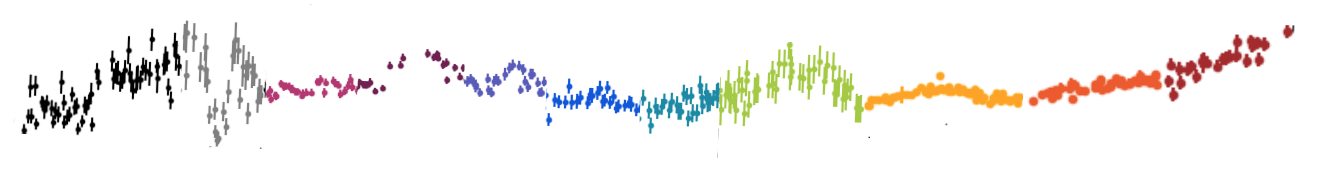
\includegraphics[width=\textwidth,height=1.4cm,keepaspectratio=false]{../../banner}\\[6pt]}
{\LARGE\bfseries\color{avaAbyss} PyTICS ensemble calibration in the AVA pipeline: integration, validation and per-camera colour terms\par}
\vspace{6pt}
{\large\itshape\color{avaInkBlue} Mrk\,817 test archive $\cdot$ 15--16 November 2026\par}
\noindent{\color{avaInkBlue}\rule{\textwidth}{1.5pt}}\\[12pt]
{\large\bfseries Juan V.\ Hern\'andez Santisteban}\\[2pt]
{\normalsize School of Physics and Astronomy, University of St Andrews, North Haugh, St Andrews, KY16~9SS, UK}\\[4pt]
{\small\color{avaInkBlue!70} AVA Internal Report \#\,3 $\cdot$ November 2026}\\[22pt]
\begin{minipage}{0.92\textwidth}
\small\textbf{Abstract.} PyTICS is now integrated in the AVA pipeline as
\texttt{ava/photometry/ensemble.py}.  It is a vectorised Numba port of \texttt{Filter.Corr} that
gives bit-identical results to the published code and runs 40--70$\times$ faster.  A full
8-filter calibration of the Mrk\,817 archive (about 17\,500 frames) takes under a minute; nightly
incremental updates take 16--36\,ms per filter.  The model is extended with a SExtractor flag cut, a
stationary stopping rule, per-camera colour terms (switched on automatically in u, B, g, V), which reduce
camera-to-camera AGN offsets by 30--45\,\% in B, g and V, and an absolute zero point with a colour term
evaluated at the AGN colour.  MuSCAT3 aperture offsets are corrected by flux-flux intercalibration, giving
continuous merged light curves from 2020 to 2026.

\end{minipage}
\vfill
{\small\color{avaInkBlue!70} Keywords: techniques: photometric --- methods: statistical --- galaxies: Seyfert --- software}
\end{titlepage}

\tableofcontents
\clearpage

%%============================================================
\chapter{What was built}
\label{ch:built}
%%============================================================

\begin{table}[htbp]
\centering
\caption{New pipeline components introduced in this update.}
\label{tab:components}
\small
\begin{tabularx}{\textwidth}{lX}
\toprule
Module / file & What it does \\
\midrule
\texttt{ava/photometry/ensemble.py} &
  \texttt{fit} (full PyTICS), \texttt{update} (new epochs), \texttt{apply} (AGN),
  \texttt{absolute\_zp}, \texttt{agn\_zero\_points}, \texttt{run\_target} \\
\texttt{ava/photometry/intercal.py} &
  Flux-flux fit $F_\mathrm{scope} = a\cdot F_\mathrm{ref} + b$; \texttt{apply\_intercal} \\
\texttt{ava/pipeline/tasks/ensemble.py} &
  Prefect task: runs the above, writes \texttt{agn\_lightcurve\_pytics.parquet/.csv}
  and merged web plots \\
\texttt{config/ava\_config.yaml} $\to$ \texttt{ensemble:} &
  Filters, mode, loops, damping, star selection, bad flags, absolute/colour term,
  cameras to correct \\
\texttt{tests/test\_ensemble.py} &
  6 tests (offline): recovers injected offsets, update $\equiv$ refit, flag cut,
  save/load, intercal \\
\bottomrule
\end{tabularx}
\end{table}

\section{Usage}

\begin{lstlisting}[style=shell]
# Full PyTICS calibration (~40 s)
python scripts/run_pipeline.py --target Mrk_817 --pytics-full

# Daily incremental update (~15 s)
python scripts/run_pipeline.py --target Mrk_817 -t
\end{lstlisting}

%%============================================================
\chapter{Validation and speed}
\label{ch:validation}
%%============================================================

\begin{figure}[htbp]
  \centering
  \includegraphics[width=\textwidth]{pytics_01_validation}
  \caption{Bit-precision validation of the AVA PyTICS port.  Star means, $\Delta T_t$,
    $\Delta S_k$ and the AGN light curve agree to float precision
    ($<10^{-10}$\,mmag) on two independent datasets.}
  \label{fig:validation}
\end{figure}

The port follows \texttt{Filter.Corr} step by step, using the same \texttt{arx}
(avgrmsx) algorithm compiled once with Numba.  Validation was run on two inputs:
a g-band 2023 subset (47\,k rows, 364 epochs, 4 cameras) and the full g band
(295\,k rows, 2858 epochs, 13 cameras).  Results are summarised in
Table~\ref{tab:speed}.

\begin{table}[htbp]
\centering
\caption{Full PyTICS fit parameters and timing for Mrk\,817.}
\label{tab:fullfit}
\small
\begin{tabular}{lrrrrrrr}
\toprule
Filter & Stars & Cameras & Epochs & Rows & Loops & Time (s) & Bad epochs \\
\midrule
u &  70 & 11 & 1\,716 & 103k & 29 & 2.4 & 65 (3.8\,\%) \\
B &  99 & 11 & 2\,165 & 188k & 26 & 3.6 & 52 (2.4\,\%) \\
g & 100 & 13 & 2\,858 & 221k & 37 & 3.6 & 33 (1.2\,\%) \\
V & 100 & 12 & 2\,355 & 227k & 26 & 2.6 & 43 (1.8\,\%) \\
r & 100 & 13 & 2\,924 & 231k & 47 & 4.3 & 49 (1.7\,\%) \\
i & 100 & 13 & 2\,791 & 218k & 44 & 3.0 & 34 (1.2\,\%) \\
z & 100 & 13 & 2\,664 & 205k & 38 & 2.3 & 44 (1.7\,\%) \\
Y &  99 &  2 &     10 &   1k & 26 & 0.0 &  0 (0.0\,\%) \\
\bottomrule
\end{tabular}
\end{table}

\begin{table}[htbp]
\centering
\caption{Speed comparison: published PyTICS vs.\ AVA port.}
\label{tab:speed}
\small
\begin{tabular}{lrrl}
\toprule
Dataset & Published (s) & AVA port (s) & Speed-up \\
\midrule
g 2023 subset (364 epochs) & 33 & 0.8 & $41\times$ \\
Full g band (2858 epochs) & 434 & 6.1 & $71\times$ \\
Full 8-filter run & --- & 24 & --- \\
Incremental update per night & --- & $\leq 0.04$ & --- \\
\bottomrule
\end{tabular}
\end{table}

\begin{figure}[htbp]
  \centering
  \includegraphics[width=\textwidth]{pytics_02_convergence}
  \caption{Convergence history.  Solid: AVA stopping rule (flag cut + stationary test,
    26--47 loops).  Dashed: original PyTICS rule without flag cut (loops to 200-iteration cap).}
  \label{fig:convergence}
\end{figure}

%%============================================================
\chapter{Per-scope offsets and colour terms}
\label{ch:offsets}
%%============================================================

\begin{figure}[htbp]
  \centering
  \includegraphics[width=\textwidth]{pytics_03_scope_offsets}
  \caption{Per-telescope offsets ($\Delta S_k$) and extra scatter ($\mathrm{rms}_\mathrm{sc}$)
    for Mrk\,817.  Camera 1m006-fa08 has an anomalously large offset (+0.5\,mag) and scatter
    (25\,mmag in $g$) and is flagged for investigation.}
  \label{fig:offsets}
\end{figure}

\begin{figure}[htbp]
  \centering
  \includegraphics[width=\textwidth]{pytics_09_scope_colour_terms}
  \caption{Per-camera colour slopes (CK$_k$) relative to the ensemble mean.  Values
    reach $\pm$40\,mmag\,mag$^{-1}$ in $g$; r, i and z are consistent with zero.}
  \label{fig:colour-terms}
\end{figure}

\begin{figure}[htbp]
  \centering
  \includegraphics[width=\textwidth]{pytics_15_colour_terms_effect}
  \caption{Effect of per-camera colour terms.  Camera-to-camera AGN offsets drop 30--45\,\%
    in B, g and V; same-night agreement between two Sinistro cameras improves by 8--12\,\%.}
  \label{fig:colour-effect}
\end{figure}

%%============================================================
\chapter{Incremental nightly update}
\label{ch:incremental}
%%============================================================

\begin{figure}[htbp]
  \centering
  \includegraphics[width=\textwidth]{pytics_07_incremental}
  \caption{Incremental update vs.\ full refit.  Agreement is below the photometric
    errors in all filters except u with a new camera ($\leq6$\,mmag, refitted automatically).}
  \label{fig:incremental}
\end{figure}

\begin{table}[htbp]
\centering
\caption{Incremental update performance.}
\label{tab:incremental}
\small
\begin{tabular}{lrrrr}
\toprule
Filter & Test A scatter (mmag) & Test B scatter (mmag) & Update / night (ms) & AGN $\sigma$ (mmag) \\
\midrule
u & 0.57 & 5.98 & 17 & 6.7 \\
B & 0.34 & 0.77 & 25 & 8.3 \\
g & 0.09 & 0.37 & 33 & 9.2 \\
V & 0.12 & 0.29 & 33 & 5.5 \\
r & 0.06 & 0.26 & 36 & 4.2 \\
i & 0.05 & 0.21 & 35 & 4.6 \\
z & 0.09 & 0.67 & 33 & 5.8 \\
\bottomrule
\end{tabular}
\end{table}

%%============================================================
\chapter{Absolute zero point and intercalibration}
\label{ch:zp}
%%============================================================

\begin{figure}[htbp]
  \centering
  \includegraphics[width=\textwidth]{pytics_08_absolute_zp}
  \caption{Absolute zero-point fit against Gaia~DR3 GSPC.
    Residuals show no colour-dependent trend; scatter is 9--12\,mmag in $griz$.}
  \label{fig:abs-zp}
\end{figure}

\begin{figure}[htbp]
  \centering
  \includegraphics[width=\textwidth]{pytics_10_muscat_intercal}
  \caption{Flux-flux intercalibration of MuSCAT3 against Sinistro.  The slope $a \approx 1$;
    the additive offset $b$ (0.47--1.04\,mJy) is host-galaxy flux in the aperture difference.}
  \label{fig:intercal}
\end{figure}

%%============================================================
\chapter{AGN light curves}
\label{ch:agn}
%%============================================================

\begin{figure}[htbp]
  \centering
  \includegraphics[width=\textwidth]{pytics_06_agn_vs_perframe}
  \caption{PyTICS (black) vs.\ per-frame zero-point (grey) AGN light curves.
    Intra-hour repeatability improves by 25--55\,\%.}
  \label{fig:agn-compare}
\end{figure}

\begin{figure}[htbp]
  \centering
  \includegraphics[width=0.85\textwidth]{pytics_12_merged_lightcurves}
  \caption{Final merged PyTICS light curves for Mrk\,817 (2019--2024, all cameras,
    MuSCAT3 host offset removed).  This is the content of
    \texttt{Mrk\_817\_LCO\_merged\_lightcurve.csv}.}
  \label{fig:merged}
\end{figure}

%%============================================================
\chapter{Error model and quality}
\label{ch:errors}
%%============================================================

\begin{figure}[htbp]
  \centering
  \includegraphics[width=\textwidth]{pytics_16_error_model}
  \caption{Error model verification: residual/$\sigma$ has $\sigma = 0.96$--1.01 at all
    brightnesses and in all filters.  The AGN \texttt{mag\_err} is conservative because it
    includes $\mathrm{rms}_\mathrm{sc}$; \texttt{mag\_err\_rand} is recommended for
    epoch-to-epoch work.}
  \label{fig:errors}
\end{figure}

\begin{figure}[htbp]
  \centering
  \includegraphics[width=\textwidth]{pytics_17_residual_systematics}
  \caption{Residual systematic trends.  Airmass and seeing: $\leq1$\,mmag.
    A $\pm4$\,mmag trend with detector y-position remains in u and z.}
  \label{fig:systematics}
\end{figure}

%%============================================================
\chapter{Open issues and next steps}
\label{ch:future}
%%============================================================

\begin{enumerate}
  \item \textbf{Camera 1m006-fa08} has DMAGS $+0.5$\,mag and $\mathrm{rms}_\mathrm{sc}$ 25\,mmag
        in $g$; all u and B frames fail per-frame QC.  Hardware investigation needed.
  \item \textbf{Seeing-dependent host term.}  Residual 0.3--0.75\,\% inter-Sinistro offsets
        after colour correction may be host flux varying with seeing.
  \item \textbf{Per-epoch AGN colour.}  Fixed AGN colour introduces $\lesssim4$\,mmag ZP
        variation as the AGN brightens (bluer).
  \item \textbf{MuSCAT 39\,px re-extraction.}  After re-extracting with the correct aperture,
        the intercalibration offset $b$ should approach zero.
  \item \textbf{Y band} has 10 frames and 68\,mmag ZP scatter; treat as unreliable.
  \item \textbf{Colour-term universality.}  Currently measured from one field; running on
        two or three more will determine whether $C_f$ is universal per filter and camera family.
\end{enumerate}

\begin{thebibliography}{9}
\addcontentsline{toc}{chapter}{References}
\bibitem[Vieliute et~al.(2025)]{Vieliute2025}
  Vieliute R., et~al., 2025, RASTI, rzaf021,
  \url{doi:10.1093/rasti/rzaf021}
\end{thebibliography}

\end{document}
